\subsection{Beam Polarimetry}
\label{sec:beam_pol}
The experimental asymmetry $\aexp$ is related 
to the corrected asymmetry by 
\begin{equation}
\aexp=\acorr_d/P_e
\label{eq:a_exp}
\end{equation}
where $P_e$ is the beam polarization. 
Three beam polarimetry techniques were available at JLab: 
A Mott polarimeter in the injector, and both a M{\o}ller
and a Compton polarimeter in the experimental hall.

\subsubsection{Mott Polarimeter}
\label{sec:mpt_exp_meth}
A Mott polarimeter \cite{Price}
is located near the injector to the first linac, where the
electrons have reached 5 MeV in energy. Mott polarimetry is based on the 
scattering of polarized electrons from unpolarized high-Z nuclei. The
spin-orbit interaction of the electron's spin with the magnetic field it sees due to its
motion relative to the nucleus causes a differential cross section

\begin{equation}\label{mottcrosssection}
\sigma(\theta) = I(\theta)
\left[1 + S(\theta){\vec P_e}\cdot \widehat{n}\right]\;\;,
\end{equation}
where $S(\theta)$ is the Sherman function
and 
$I(\theta)$ is the spin-averaged scattered intensity
\begin{equation}
I(\theta)= \frac{Z^2 e^4}{4m^2\beta^4 c^4 \sin^4(\theta/2)} \left[1 - \beta^2\sin^2(\theta/2)\right](1 - \beta^2) \;\;\; .
\end{equation}
 The unit vector ${\widehat n}$ is normal to the scattering plane, defined by
$
\widehat n = (\vec k \times \vec k')/\vert \vec k \times \vec k' \vert
$
where $\vec k$ and $\vec k'$ are the electron's momentum before and
after scattering, respectively. Thus $\sigma(\theta)$ depends on the electron beam polarization $P_e$.
Defining an asymmetry
\begin{equation}
A(\theta) = \frac{N_L - N_R}{N_L + N_R} \; ,
\end{equation}
where $N_L$ and $N_R$ are the number of electrons scattered to the left and
right, respectively, we have 
\begin{equation}
A(\theta) = P_e \; S(\theta) \;,
\end{equation}
and so knowledge of the Sherman function $S(\theta)$
allows $P_e$ to be extracted from the measured asymmetry
with a precision of 3\% \cite{Sinclair1},\cite{HAPPEXsff}.
The Mott polarimeter is also used for setting up and verifying
the transversely-polarized beam used for systematic checks.

\subsubsection{M{\o}ller Polarimeter}
\label{sec:moller_method}

A M{\o}ller polarimeter measures the beam polarization
via measuring the asymmetry in
$\vec e, \vec e$ scattering, which depends on the
beam and target polarizations $P^{\rm beam}$ and $P^{\rm target}$, 
as well as on the
analyzing power $\ath_m$ of M{\o}ller scattering:

\begin{equation}
\label{moller_asy}
         \aexp_m = 
            \sum_{i=X,Y,Z} (\ath_{mi}\cdot{}{P}^{\rm targ}_{i}\cdot{}{P}^{\rm beam}_{i}) ,
\end{equation}
where $i = X,Y,Z$ defines the projections of the polarizations
($Z$ is parallel to the beam, while $X-Z$ is the scattering plane).
The analyzing powers $\ath_{mi}$ depend on 
the scattering angle $\theta_{\rm CM}$ in the
center-of-mass (CM) frame 
and are calculable in QED.
The longitudinal analyzing power is
\begin{equation}
\label{eq:moller_apower}
\ath_{mZ} = - \frac{ \sin^2 \theta_{\rm CM} 
( 7 + \cos^2 \theta_{\rm CM}) }
{ {(3 + \cos^2 \theta_{\rm CM})}^2 }.
\end{equation}

The absolute values of $\ath_{mZ}$ reach the maximum of 7/9 
at $\theta_{\rm CM}=90^{\circ}$. 
At this angle the transverse analyzing powers are $\ath_{mX}=-\ath_{mY}=\ath_{mZ}/7$.

The polarimeter target is a ferromagnetic foil
magnetized in a magnetic field of 24 mT along its plane.
The target foil can be oriented at various angles
in the horizontal plane providing both
longitudinal and transverse polarization
measurements.  The asymmetry is measured
at two target angles ($\pm 20^{\circ}$) 
and the average taken, which cancels
transverse contributions and reduces
the uncertainties of target angle measurements.
At a given target angle two sets of measurements
with oppositely signed target polarization
are made which cancels some false asymmetries
such as beam current asymmetries.  The target
polarization was (7.95 $\pm$ 0.24)\%.

The M{\o}ller-scattered electrons were
detected in a magnetic spectrometer 
consisting
of three quadrupoles and a dipole \cite{A-NIM}.
The spectrometer selects electrons in a
bite of $75^{\circ} \le \theta_{\rm CM} \le
105^{\circ}$ and $-5^{\circ} \le \phi_{\rm CM}
\le 5^{\circ}$ where $\phi_{\rm CM}$ is
the azimuthal angle.  The detector consists
of lead-glass calorimeter modules in two 
arms to detect the electrons in coincidence.
More details about the M{\o}ller polarimeter
are published in \cite{A-NIM}.  The total
systematic error that can be achieved is
3.2\% which is dominated by uncertainty in
the foil polarization.

\subsubsection{Compton Polarimeter}
\label{sec:cpt_exp_meth}

The Compton polarimeter ~\cite{Baylac} \cite{Neyret} ~\cite{megan}
is based on scattering of the polarized electron beam from
a polarized laser in a beam chicane.
The backscattered photons are detected in a GsO crystal ~\cite{megan}.

The experimental
asymmetry $\aexp_c=(N^+-N^-)/(N^++N^-)$ is measured, where
$N^+\, (N^-)$ refers to Compton counting rates for right (left)
electron helicity, normalized to the beam intensity. This asymmetry is
related to the electron beam polarization via
\begin{equation}
P_e=\frac{\aexp_c}{P_\gamma \ath_c}
\label{eq:a_expc}
\end{equation}
where $P_\gamma$ is the photon polarization and $\ath_c$ the analyzing
power.  At typical JLab energies (a few GeV), the Compton cross-section
asymmetry is only a few percent.
To compensate for this, a Fabry-Perot cavity
\cite{Jorda} is used to amplify the photon density of a standard
low-power laser at the integration point. An average power of 1200 W
is accumulated inside the cavity with a photon beam waist of the
order of 150 $\mu$m and a photon polarization above 99\%, monitored
online at the exit of the cavity \cite{Falletto}.


\subsubsection{Beam Polarization Results}
\label{sec:cpt_exp_meth}

During our experimental run, the M{\o}ller polarimeter the entire time,
while the Compton polarimeter initially suffered from a high background
and only produced results in the last three weeks of the run.
Figure ~\ref{fig:moller} shows the M{\o}ller polarimetry measurements during
our experiment, and figure ~\ref{fig:compton} shows the Compton measurements
together with M{\o}ller measurements that were taken during the time period.

\begin{figure}[!ht]
\centering
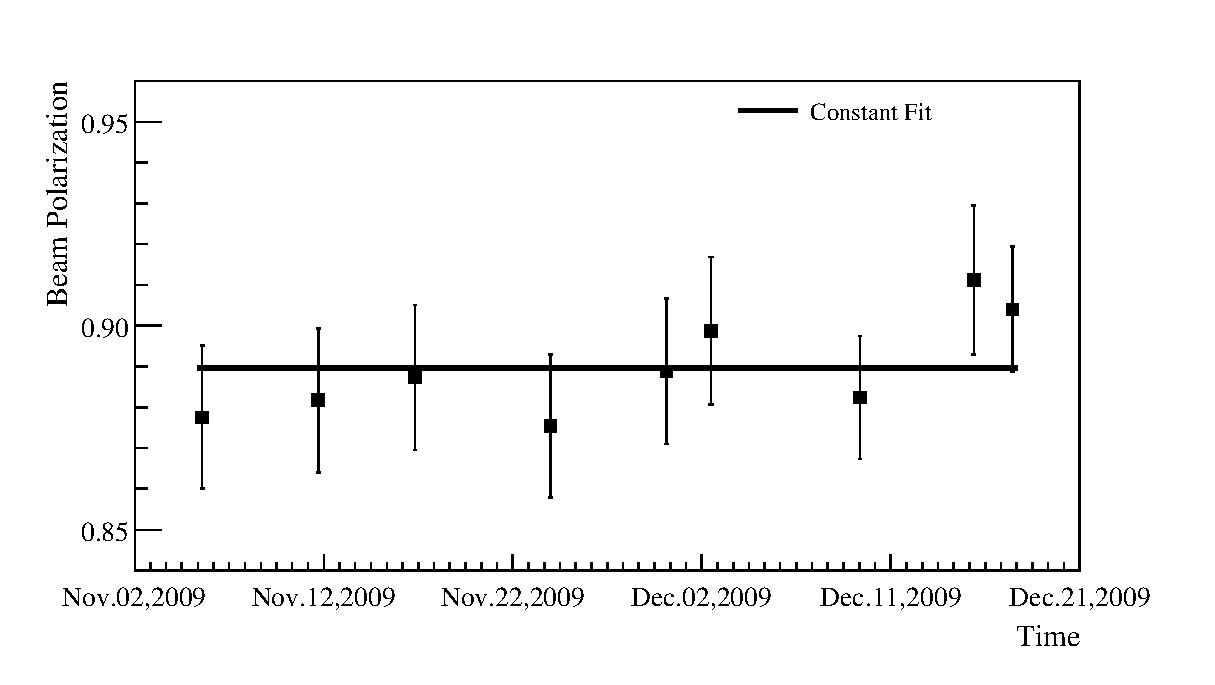
\includegraphics{RM/mollerpol.eps}
\caption{Polarization history from the M{\o}ller polarimeter measurements. 
The error bars include systematic error.}
\label{fig:moller}
\end{figure}


\begin{figure}[!ht]
\centering
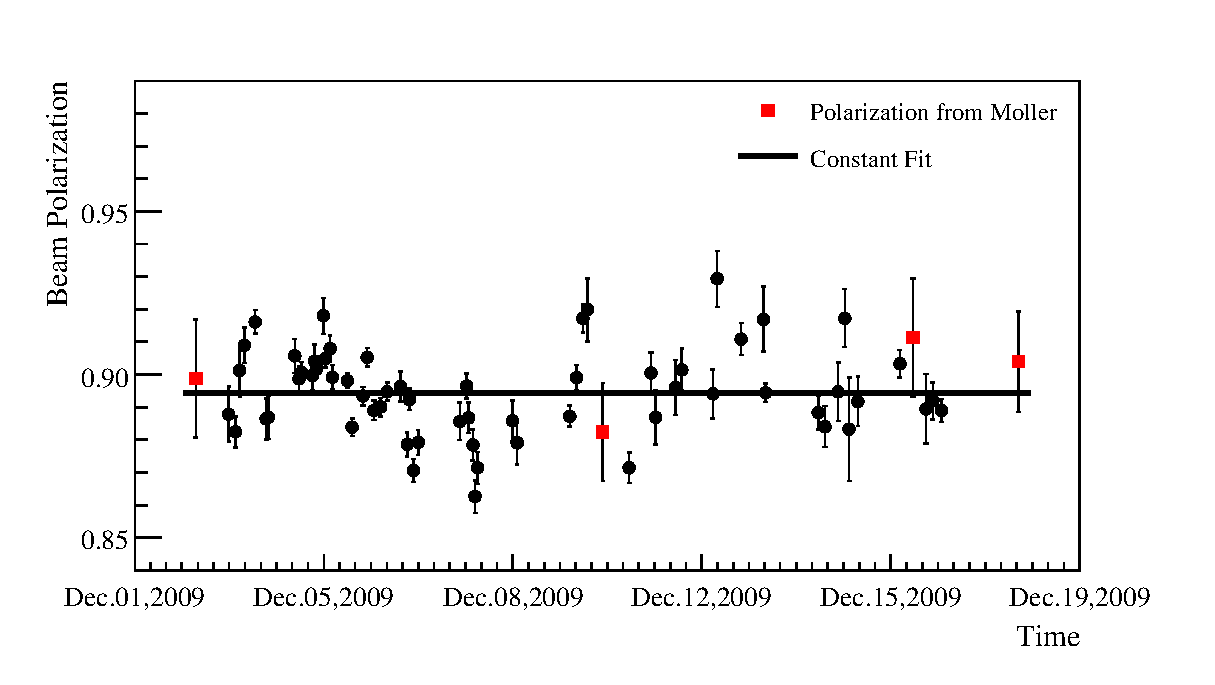
\includegraphics{RM/comptonpol.eps}
\caption{Polarization history from Compton measurement (round points), 
together with Moller measurements (square points) during the same time. 
The error bars for Compton are statistical only, while for Moller include systematic.}
\label{fig:compton}
\end{figure}

The average beam polarization from constant fit is $88.97\%$ for M{\o}ller and $89.45\%$ for Compton. 
The way that we apply the beam polarization correction is as following:

\begin{enumerate}
\item{ \label{it:moller_cor} When there's no Compton measurements (before Dec 2), 
only M{\o}ller results are used. Each Moller data point is used for the 
consecutive days until the next data point is available.}

\item{ When there are both Compton and M{\o}ller results (after Dec 2), 
the Compton data are averaged first and then this average is 
averaged with each Moller point. These results are applied 
for correction in the same way as \ref{it:moller_cor}.}

\item {The beam polariztion is corrected run by run. }
\end{enumerate}

The run-by-run averaged beam polarization corrections are shown in 
table ~\ref{tab:polarimeter} for the different kinematics and
spectrometers (Left/Right HRS).

\begin{table}[!ht]
  \begin{center}
    \begin{tabular}{c|c|c|c}
      \hline\hline
                    &  Left Kine 1   &    Left Kine 2    & Right Kine 2 \\ \hline
      Polarization  &  $88.18\%$      &    $89.29\%$       & $88.73\%$  \\ \hline
      Uncertainty   &  $1.76\%$      &    $1.19\%$       & $1.50\%$  \\ \hline
      \hline
    \end{tabular}
  \end{center}
\label{tab:polarimeter}
\end{table}


